\capitulo{1}{Introducción}

% Descripción del contenido del trabajo y del estructura de la memoria y del resto de materiales entregados.

El desarrollo de software es una actividad que puede ser enormemente compleja al poder desarrollar proyectos de gran envergadura que impliquen a muchas personas y entidades trabajando con diferentes herramientas y con variados patrones de organización \cite{jacobson_proceso_2000}. Esta complejidad existe a nivel técnico ya que se requiere que se cumplan los requisitos establecidos funcionales pero es necesario que también se cumpla con los no funcionales como pueden ser la seguridad, la posibilidad de actualización, la escalabilidad de la arquitectura elegida, los tiempos de carga, etc.
Además, esta complejidad existe también a nivel organizativo, es necesario que los jefes de proyecto sean capaces de organizar a los equipos y el trabajo a realizar de forma que se optimice tanto el tiempo como los recursos económicos disponibles.

Para poder salvar esta complejidad y que los jefes de proyecto sean capaces de llevar a cabo su tarea de optimización de los recursos se han creado diferentes modelos que permiten definir las actividades y tareas realizadas en los proyectos de forma organizada y lo más sencilla posible. Entre estos modelos destaca \textit{\textbf{Unified Process (UP)}} \cite{jacobson_proceso_2000} donde se definen las siguientes tareas en un proyecto: 

\begin{itemize}
	\item Captura de requisitos.
	\item Análisis
	\item Diseño
	\item Implementación
	\item Prueba
\end{itemize}

Estas diferentes tareas o fases de realizan de forma iterativa e incremental, es decir, tras la fase de prueba se comprueba que no existen nuevos requisitos y se repite todo el proceso. Cada una de estas iteraciones ha de resultar en un entregable o artefacto a ser posible funcional.

Este desarrollo iterativo incremental está también reflejado en otras metodologías de trabajo como son las de desarrollo ágil como \textit{Scrum}, \textit{Lean} o \textit{eXtreme Programming}.


Para poder llevar a cabo este desarrollo iterativo y de forma colaborativa, entre varios desarrolladores, es necesario disponer de herramientas que permitan la gestión de los productos software como el proceso de desarrollo del equipo. Estas herramientas son los repositorios de software que son espacios centralizados donde se almacena, organiza, mantiene y difunde información digital, habitualmente archivos informáticos, que pueden contener trabajos científicos, conjuntos de datos o software\footnote{\url{https://es.wikipedia.org/}}. 

Las herramientas de control de repositorios o forjas de proyectos software han evolucionado con los años y tienen muchas más funcionalidades, además del control de cambios de los archivos, se centran en fomentar el desarrollo colaborativo y la interacción entre desarrolladores.
Entre dichas funcionalidades podemos nombrar el control de versiones, el control de los archivos de forma colaborativa, almacenándose tanto los propios archivos como las interacciones entre los miembros del equipo que los manipulan, sistemas de revisión de calidad, sistemas de control de incidencias (o \textit{issues}) o sistemas de integración y despliegue continuo denominados \textit{CICD} (\textit{Continuous delivery - Continuous deployment}).
Entre estas herramientas podemos destacar en la actualidad por ser las más usadas:  \textit{GitHub}\footnote{\url{https://github.com/}}, \textit{GitLab}\footnote{\url{https://about.gitlab.com/}} o \textit{Bitbucket}\footnote{\url{https://bitbucket.org/}}) aunque existen otras como \textit{SourceForge}\footnote{\url{https://sourceforge.net/}}.

Estas herramientas están en continua evolución desarrollando nuevas funcionalidades para mejorar la experiencia de los desarrolladores y los gestores de proyectos y permiten integración con terceros para ofrecer aquellas características que aún no ofrecen.
En el orden de las metodologías ágiles las diferentes plataformas están avanzando mucho ofreciendo por ejemplo \textit{GitLab} el módulo \textit{GitLab Issues}\footnote{\url{https://docs.gitlab.com/ee/user/project/issues/}}) o  
\textit{GitHub} ofreciendo \textit{GitHub Issues}\footnote{\url{https://docs.github.com/en/issues/tracking-your-work-with-issues/about-issues}} (mejorado con \textit{ZenHub}\footnote{\url{https://www.zenhub.com/}}) que es la solución utilizada en este proyecto.

Estas herramientas generan una enorme cantidad de información de los proyectos y del proceso de desarrollo. En la actualidad uno de los aspectos del desarrollo de software que más interés despierta y en el que se realizan más avances es en la gestión de esta información ya que, cuanto más se optimice dicha gestión de la información, antes se pueden detectar los fallos en el proceso de desarrollo para optimizarlo.
Este es el campo de trabajo de los jefes de proyecto, el correcto control sobre el proceso de desarrollo y el producto creado. Es por esto crucial que exista una manera de medir si se está realizando correctamente dicho proceso o no.
Para ello existen las control y de predicción \cite{sommerville_ingenierisoftware_2002}. Las primeras se refieren al proceso de desarrollo, y las segundas al producto, en el presente TFG nos centraremos fundamentalmente en las primeras.

Es claro que el resultado de un proyecto dependerá del proceso de desarrollo seguido y su calidad. Esto es explicado, por ejemplo, por Sommerville en \textit{Ingeniería de software} \cite{sommerville_ingenierisoftware_2002} y que cuanto mejor sea este proceso mejores resultados se obtendrán a la finalización de los proyectos.

Este presente TFG pretende profundizar en este punto, mejorar la calidad de los procesos de desarrollo,  implementado medidas automáticas del proceso desarrollado en GitHub. Se implementa una nueva iteración sobre \textit{\textbf{Evolution Metrics Gauge}}, un software para calcular métricas de control\footnote{También llamadas métricas de proceso o métricas de evolución.}.
Dicho software ha sido desarrollado en un TFG previo titulado \textit{\textbf{Evolution Metrics Gauge - Comparador de métricas de evolución en repositorios software}} \cite{TFGPrevio}. Este software consiste en una aplicación web escrita en lenguaje \textit{Java} que toma como entrada un conjunto de repositorios públicos o privados de \textit{GitLab} y calcula métricas de evolución que permiten comparar los proyectos.
En esta nueva iteración se extiende la funcionalidad a repositorios de \textit{GitHub}, se añaden nuevas métricas y se implementan diferentes mejoras. Podemos ver las diferencias entre las interfaces de ambas iteraciones en las figuras \ref{fig:M1_ComparativaNuevaIteracion} y \ref{fig:M1_ComparativaIteraciónPrevia}

\begin{figure}[!h]
	\centering
	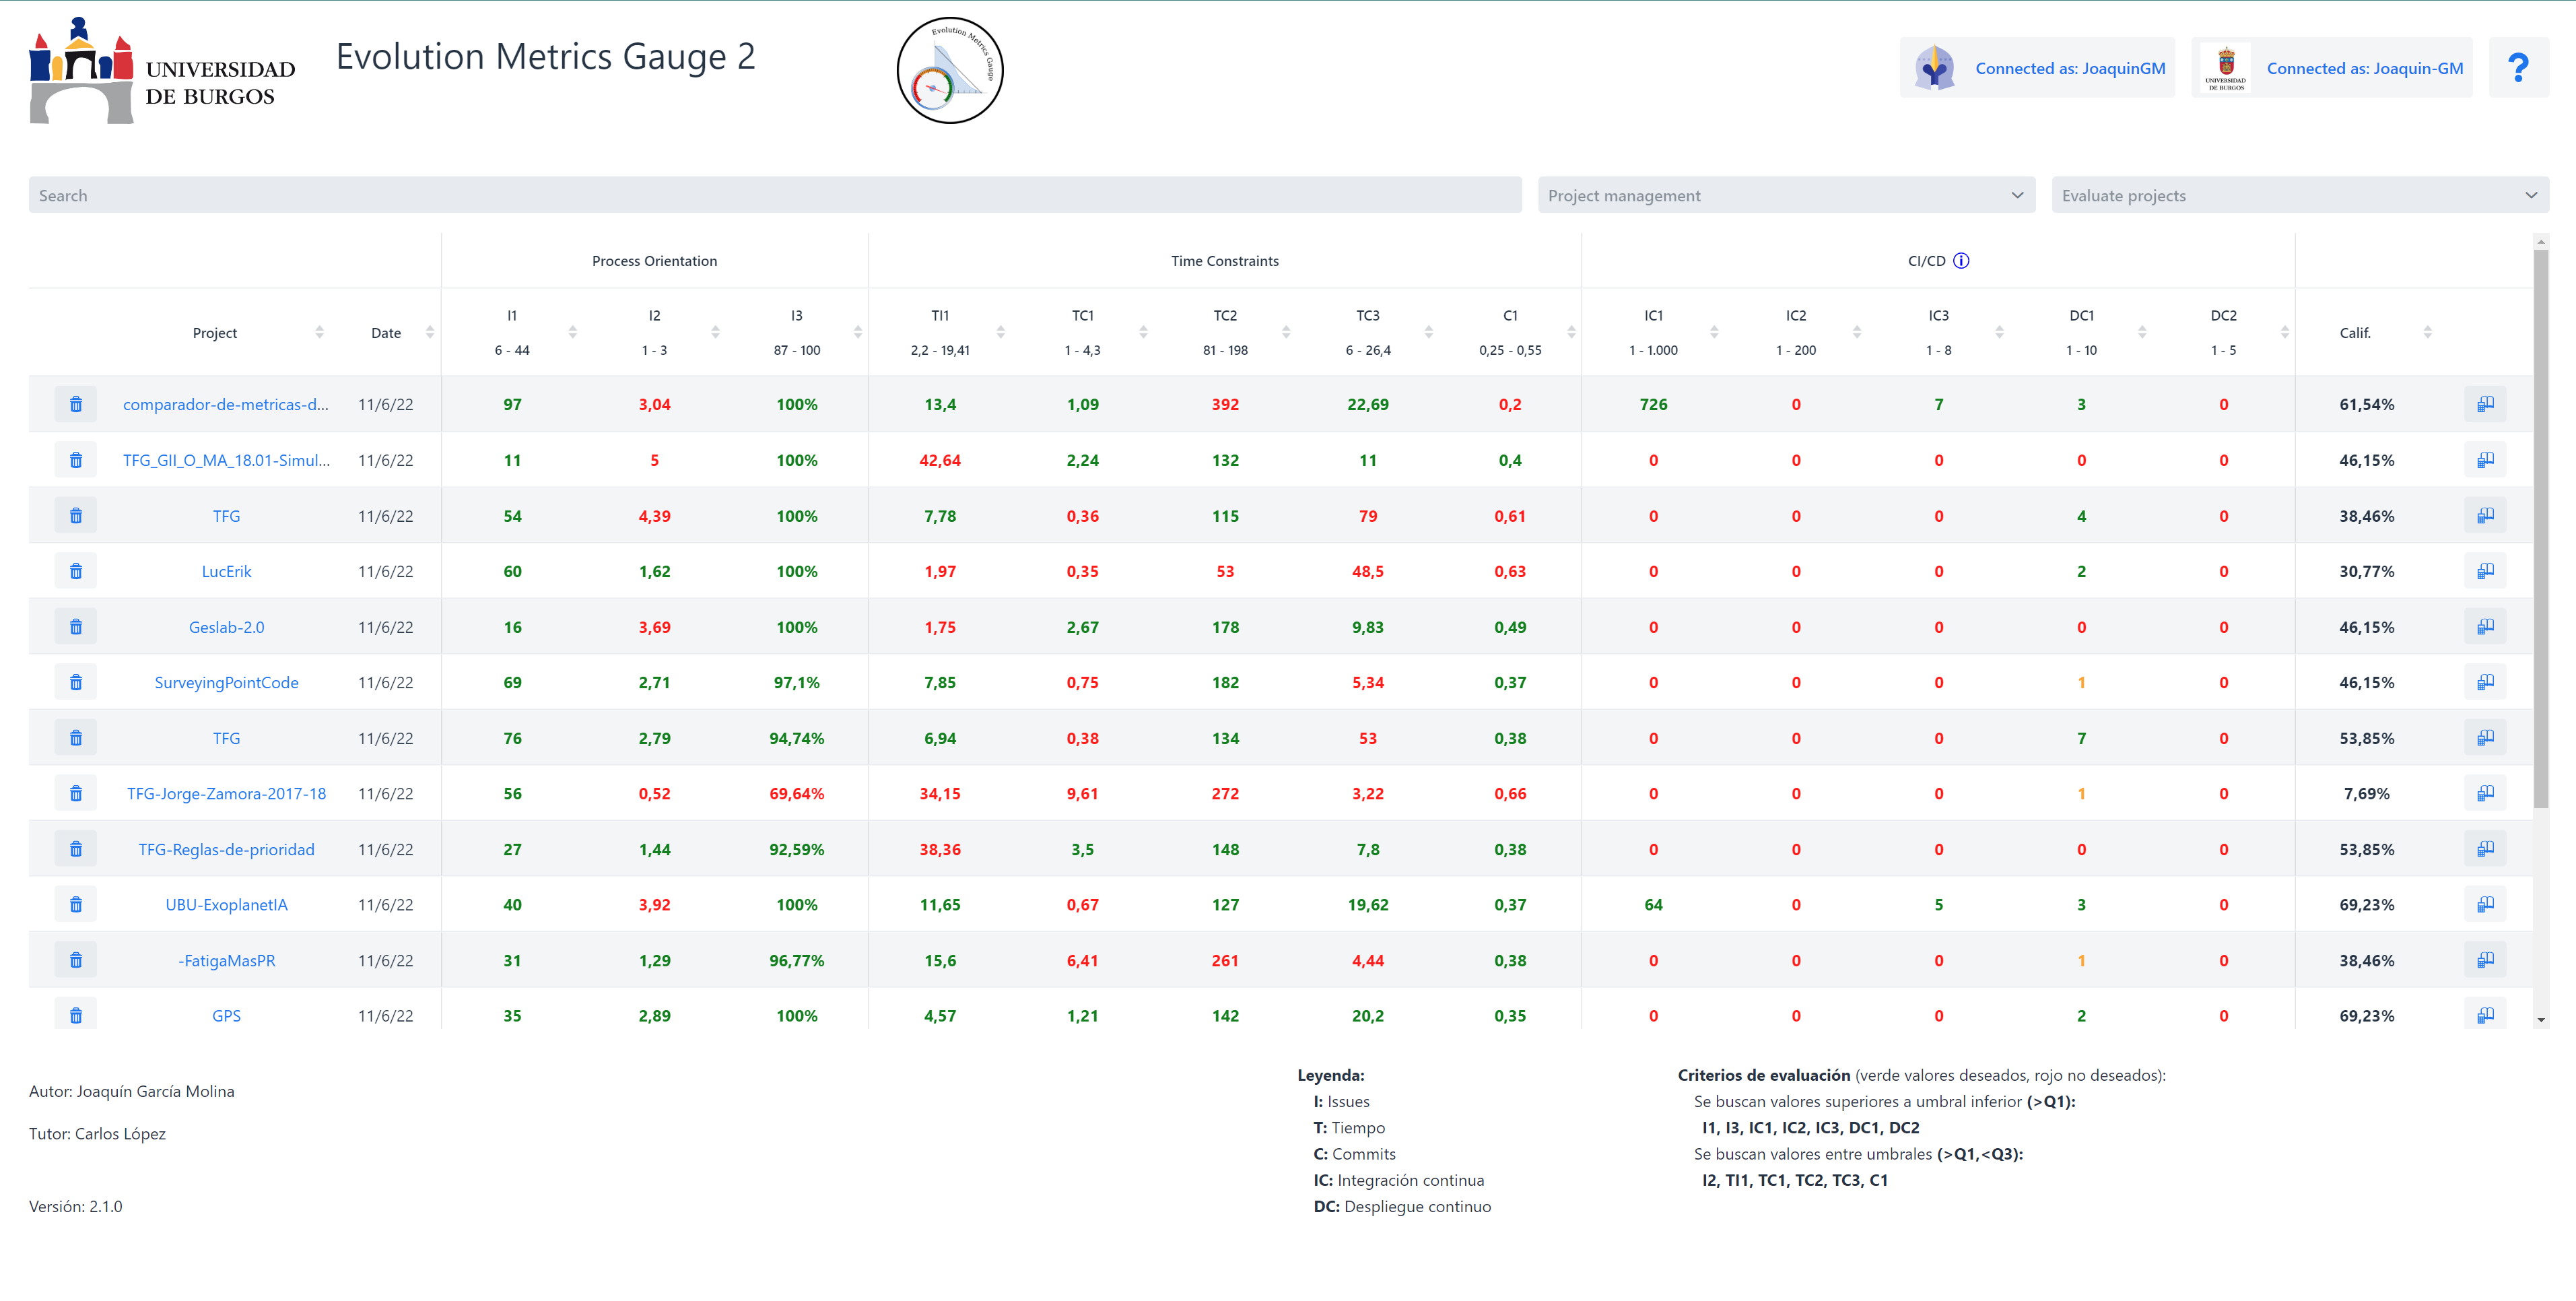
\includegraphics[width=1\textwidth]{M1_ComparativaNuevaIteracion}
	\caption{Nueva versión generada en este TFG de \textit{Evolution Metrics Gauge - Comparador de métricas de evolución en repositorios software}}\label{fig:M1_ComparativaNuevaIteracion}
\end{figure}
\FloatBarrier


\begin{figure}[!h]
	\centering
	\includegraphics[width=1\textwidth]{M1_ComparativaIteraciónPrevia}
	\caption{Primera iteración de \textit{Evolution Metrics Gauge - Comparador de métricas de evolución en repositorios software}}\label{fig:M1_ComparativaIteraciónPrevia}
\end{figure}
\FloatBarrier

\newpage
\section{Estructura de la memoria}

La presente memoria tiene la siguiente estructura\footnote{Se parte de lap lantilla \textit{LaTex} proporcionada en \url{https://github.com/ubutfgm/plantillaLatex}}:

\begin{description}
	\tightlist
	\item[Introducción.] Introducción. Estructura de la memoria y anexos.
	\item[Objetivos del proyecto.] Objetivos que busca alcanzar el proyecto.
	\item[Conceptos teóricos.] Definiciones de los conceptos empleados en el proyecto.
	\item[Técnicas y herramientas.] Técnicas y herramientas utilizadas durante el desarrollo del proyecto.
	\item[Aspectos relevantes del desarrollo.] Aspectos destacables durante el proceso de desarrollo del proyecto.
	\item[Trabajos relacionados y \textit{debt process}.] Desarrollos relacionados y deuda técnica asociada a proceso.
	\item[Conclusiones y líneas de trabajo futuras.] Conclusiones tras la realización del proyecto y posibilidades de mejora o expansión.
\end{description}

Se incluyen también los siguientes anexos:

\begin{description}
	\tightlist
	\item[Plan del proyecto software.] Planificación temporal y estudio de la viabilidad del proyecto.
	\item[Especificación de requisitos del software.] Análisis de los requisitos.
	\item[Especificación de diseño.] Diseño de los datos, diseño procedimental y diseño arquitectónico.
	\item[Manual del programador.] Aspectos relevantes del código fuente.
	\item[Manual de usuario.] Manual de uso para usuarios que utilicen la aplicación.
\end{description}
